\documentclass[dvipdfmx]{jarticle}
\pagestyle{empty}
\usepackage{tikz}
\usetikzlibrary{shapes,calc,arrows.meta}
\begin{document}
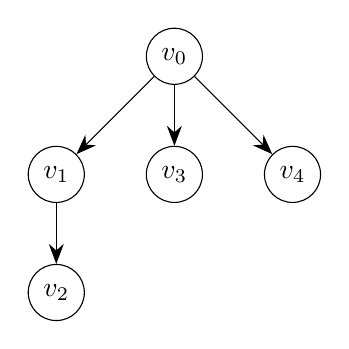
\begin{tikzpicture}
    \node[draw,circle] (v0) at (0,0) {$v_0$};
    \node[draw,circle] (v1) at (-1.5,-1.5) {$v_1$};
    \node[draw,circle] (v2) at (-1.5,-3) {$v_2$};
    \node[draw,circle] (v3) at (0,-1.5) {$v_3$};
    \node[draw,circle] (v4) at (1.5,-1.5) {$v_4$};
    \path[-{Stealth[scale=1.5]}] (v0) edge (v1);
    \path[-{Stealth[scale=1.5]}] (v1) edge (v2)
    (v0) edge (v3) (v0) edge (v4);
\end{tikzpicture}
\end{document}